\documentclass[conference,compsoc]{./IEEEtran/IEEEtran}

%% Configure which sections are included:
%\newcommand*{\OPTIONAL}{}


% *** CITATION PACKAGES ***
% IEEE Computer Society needs nocompress option
% requires cite.sty v4.0 or later (November 2003)
\usepackage[nocompress]{cite}

% *** ALIGNMENT PACKAGES ***
\usepackage{array}

% *** SUBFIGURE PACKAGES ***
\usepackage[caption=false,font=footnotesize,labelfont=sf,textfont=sf]{subfig}
% The latest version and documentation of subfig.sty can be obtained at:
% http://www.ctan.org/pkg/subfig

% correct bad hyphenation here
\hyphenation{op-tical net-works semi-conduc-tor}



%\usepackage{hyperref}

\usepackage{graphicx}
\DeclareGraphicsExtensions{.png,.jpg,.pdf,.eps}

\usepackage{pgfplots}
\pgfplotsset{compat=1.9}


\begin{document}

\title{Raft Distributed Consensus Algorithm over\\ WebRTC (Web Real-Time Communication)}

\author{\IEEEauthorblockN{Joel Martin}
\IEEEauthorblockA{Department of Computer Science and Engineering\\
University of Texas at Arlington\\
Arlington, TX 76010\\
Email: joel@martintribe.org}
\and
\IEEEauthorblockN{David Levine}
\IEEEauthorblockA{Department of Computer Science and Engineering\\
University of Texas at Arlington\\
Arlington, TX 76010\\
Email: levine@cse.uta.edu}}

\maketitle

\begin{abstract}
We describe the creation of a browser-based distributed peer-to-peer
application using WebRTC, PeerJS and Raft.js. WebRTC is a protocol
that modern browsers have begun to integrate which enables
browser-to-browser communication. PeerJS is a WebRTC client library
and extensible signaling server. Raft.js is an implementation in
JavaScript of the Raft distributed consensus protocol. These
technologies are combined to create a chat application that guarantees
a shared, consistent and linearized view of the chat history without
relying on a single centralized server for communication. We also
create a series of automated tests using the SlimerJS browser
automation tool and use them to show the correctness of the chat
application and also to measure the performance and scalability of the
application for various cluster sizes.
\end{abstract}

\section{Introduction}
In the past few years, browsers have quickly evolved from document
rendering engines into powerful platforms for building sophisticated
applications. Modern browsers are integrating new protocols for
communication including WebSockets for full-duplex browser-to-server
communication \cite{websockets:rfc6455} and WebRTC for direct
browser-to-browser communication \cite{webrtc:feb2015}. These new
capabilities enable software developers to treat web applications as
first class participants in distributed network applications.

These new browser capabilities also bring with them the traditional
challenges of building reliable distributed applications, such as:
concurrency, security, scalability, naming, discovery, replication,
relocation, etc. The solutions to many of these challenges involve
the proper management of distributed state. Distributed consensus is
one category of distributed state management in which multiple nodes
must come to agreement on the state of a single value or set of values. % TODO/CITE
The grandparent of distributed consensus algorithms is the Paxos
algorithm described by Leslie Lamport \cite{paxos:lamport98}. However,
Paxos has been notoriously difficult to understand and to implement
correctly \cite{paxos:chandra07}. Raft is a more recent distributed
consensus algorithm that aims for understandability and practicality
of implementation \cite{raft_thesis:ongaro14}.

In this paper we will describe an implementation of the Raft protocol
in a browser context using WebRTC as the communication channel. We
will describe the results of the implementation and look at some of
the unique challenges (and opportunities) we encountered with the
implementation. We will also explore some ideas for further study.

\section{Motivation/Use Cases}
The traditional use of distributed consensus is in the data-center
(private or cloud based), often as the core coordination component
of a replicated data-storage system. %TODO/CITE
In these examples, the set of nodes that compose the cluster tend to
be fairly static and changes to cluster membership are usually for the
purpose of replacing nodes. Changes to the long-term size of the
cluster are uncommon. %TODO/CITE

Most existing distributed browser applications are extensions of the
data-centric model in which browsers connect to load-balanced web
servers which are in close network proximity to the distributed
consensus cluster. %TODO/CITE
The backend web servers deliver the web application to the browser and
also serve as the conduit for all browser-to-browser communication and
state management.

However, requiring application messages and application state to
traverse the back-end servers is not always desirable for various
reasons, including the following:

\begin{enumerate}
\item \emph{security (privacy)}: application state and user messages
    may need to traverse directly from browser to browser rather than
    traversing a server.
\item \emph{locality}: the nature of the application may allow
    clusters of applications that are nearby on a network (e.g.
    intranet) to communicate and coordinate directly rather than
    passing all messages and state through a server back-end which may
    be considerably more remote.
\item \emph{bandwidth and scale}: a distributed browser based
    application may be able to avoid expensive bandwidth into and out
    of the backend data-center by passing messages and state directly
    between browsers.  Depending on the design of the application this
    may also enable better scalability then a more centralized model.
\end{enumerate}

%TODO: better lead in to this paragraph from above
Here are some specific use cases in which Raft over WebRTC may be
applicable:

\begin{enumerate}
\item \emph{Consistent order secure chat}: a chat room system where
    all users see the same message history but the messages never
    traverse a central server and there is no central arbiter
    of truth. The application code itself may still be delivered from
    a central web service. This use case was implemented
    for this paper.
\item \emph{Private multiuser document editing/whiteboard system}:
    Google Docs, among other examples, has demonstrated a powerful
    model for collaborative document creation. However, these systems
    all use a centralized servers to coordinate shared state and
    handle browser-to-browser communication. %TODO/CITE
    Using Raft over WebRTC could enable applications with similar
    functionality but without the central coordination and
    communication.
\item \emph{Browser based network games}: most network games have
    certain states that must be agreed upon by all nodes (e.g. avatar
    dead or alive, etc). This can be achieved with Raft over WebRTC
    without requiring any data to traverse a central server. In
    addition to reducing browser to server bandwidth requirements,
    this may also allow lower latency gaming if game instances are
    partitioned into clusters based on latency.
\end{enumerate}

\section{Background}

\subsection{Raft}

Raft is a new distributed consensus algorithm designed to be
understandable and practical without sacrificing safety and
correctness. The Raft algorithm implemented and described in this
paper is based on Diego Ongaro's dissertation ``Consensus: Bridging
Theory and Practice" \cite{raft_thesis:ongaro14}.

The Raft algorithm breaks the problem of consensus into three core
sub-problems: leader election, log replication, and safety
\cite[Section~3]{raft_thesis:ongaro14}. A full Raft system must also
address: cluster membership changes
\cite[Section~4]{raft_thesis:ongaro14}, log compaction
\cite[Section~5]{raft_thesis:ongaro14}, and client interaction
\cite[Section~6]{raft_thesis:ongaro14}. The Raft protocol is based on
the concept of a distributed transaction log. Entries in the log
represent a sequence of commands that will be applied to an internal
state machine. If all members of the Raft cluster have the same log
entries, then their state machine on each node will have exactly the
same state. Each node of a Raft cluster can be in one of three states:
follower, candidate, or leader. The responsibility of the leader is to
accept new transaction log entries and then replicate these entries in
the same order to all other members of the cluster. The leader is the
only member of the cluster that may make changes to the transaction
log. In order to maintain leadership, the leader sends heartbeat RPCs
to all the followers in the cluster.  Followers that do not receive
a heartbeat RPC within a certain time period become candidates and
attempt to be elected by the other nodes as the new leader of the
cluster \cite[p.~12]{raft_thesis:ongaro14}.

\subsubsection{Leader Election}

Each node of the Raft cluster maintains an ordinally increasing
current term value. When a Raft follower node does not receive
a heartbeat from a leader within a locally randomized election timeout
period, it transitions to candidate state, votes for itself, increases
its current term value by one and sends a requestVote RPC (with the
new term) to all the other nodes in the cluster. When a node receives
a requestVote RPC with a term that is greater than its own it will
become a follower (if not already), update its term to the new term,
and send a RPC response back that indicates a vote for that candidate.
However, a node may only vote for one candidate in a given term. If
a candidate receives votes from more than half of the cluster, then it
immediately becomes a leader and sends out a appendEntries RPC to
confirm leadership and reset the election timers on all the other
nodes \cite[Section~3.4]{raft_thesis:ongaro14}.

\subsubsection{Log Replication}

Each Raft node maintains a transaction log. The entries in the
transaction log each contain a term value in addition to the action to
apply to the state machine. Each node also keeps track of the most
recent log entry which is known to be committed (exists in the log of
more than half the nodes in the cluster).

When a new leader is elected, it begins sending appendEntries RPCs
to other nodes in the Raft cluster. These RPC messages contain
information about the state of its transaction log: index and term of
the latest entry, and the most recently committed entry. If the node
does not have an entry matching the most recent entry on the leader,
then it replies with false to indicate that its log is not up to
date. The next appendEntries RPC that the leader sends to that
node will contain the next oldest index and term. This will continue
until the leader discovers the latest log entry which is in agreement
(the node may not have any entries if it is new). Then the leader will
begin to propagate entries to the node in subsequent appendEntries
RPCs until the node is caught up. The leader continues sending
empty appendEntries as heartbeat RPCs to all the nodes until it
receives a new entry in its transaction log from a client
\cite[Section~3.5]{raft_thesis:ongaro14}.

\subsubsection{Safety}

In order to ensure that each state machine on every node executes
exactly the same commands in exactly the same order, the Raft system
provides safety guarantees. In particular, there are some restrictions
on whether a Raft node is actually eligible to become a leader, based on
the state of its transaction log compared to other node transaction
logs. A Raft node will only vote for a candidate if the candidate has
a log that is more up-to-date than the voter. A log entry with a later
term is always more up-to-date. If the log entries have the same term,
then the entry with a higher index is more up-to-date. In addition,
a Raft leader may not consider entries from a previous term to be
committed until it has committed at least one entry from its own
term
\cite[Section~3.6]{raft_thesis:ongaro14}.

Raft nodes must also persist certain properties to durable storage
before sending or receiving any RPCs. The properties that must be
persisted are: current term, current vote for this term (if any), and
either the full transaction log or the state machine plus any
unapplied transaction log entries
\cite[Section~3.8]{raft_thesis:ongaro14}.

\subsubsection{Membership Changes}

Raft leverages the replicated transaction log to accomplish live
cluster membership changes. Membership changes are accomplished by
adding or removing one Raft node at a time using special add/remove
log entries. As soon as the new entry is added to the log it becomes
effective on that node without waiting for the entry to be fully
committed across the cluster. However, a new cluster change entry may
not be added to the log until the previous one is committed. Once the
change entry is committed, the initiator of the change is notified,
removed servers can be shut down and another change entry may be added
to the log \cite[Section~4]{raft_thesis:ongaro14}.

\subsubsection{Log Compaction}

In order to keep the replicated transaction log from growing
indefinitely, Raft nodes should periodically compact their logs. There
are many different ways to accomplish log compaction and the best way
will depend on application requirements and on the specific nature of
the distributed state machine. For example, if the state machine is
simply a single shared counter, then any log entries before the most
recently committed entry may be safely discarded.
The simplest and most generic solution is often to provide some way of
snapshotting the entire state machine (including the term and log
index it represents) to disk at which point all previously applied log
entries can be discarded. Snapshotting the state machine also means
that the implementation must provide a way for the leader to serialize
and send the current state machine to other nodes if their transaction
log is too old (e.g. when a new node is added)
\cite[Section~5]{raft_thesis:ongaro14}.

\subsubsection{Client Interaction}

Clients of the Raft cluster are able to interact with the distributed
state machine by sending RPCs to the leader in order to add command
entries to the transaction log. Clients first find the address of any
node in the cluster either via broadcast, via an external directory
service, or directly provided by the user. Once the client discovers
a node of the cluster, that node can either forward messages directly
to the leader node (if it is not the leader) or it can reject client
requests with a response indicating the address of the leader where
client requests should be redirected
\cite[Section~6.2]{raft_thesis:ongaro14}.

The Raft protocol also provides strict linearizable semantics for
client commands/requests (reads and writes) for applications that
require it.
In order to accomplish this, each client is given a unique ID, and the
client assigns a unique serial number to each command.  This prevents
a single client command from being applied twice (leader crash,
network duplication) or lost (packet loss)
\cite[Section~6.3]{raft_thesis:ongaro14}.

Linearizability is important not just for writes/updates to the state
machine, but also for reads, which means that read requests must also
be entered as transactions in the log and committed to more than half
the Raft nodes before the leader can respond to the client. If reads
bypass the transaction log then those reads are serializable but not
necessarily linearizable. For example, a leader may have been deposed
and not realize it if the cluster is partitioned which could result in
reads of stale data (the leader of the larger partition may have
already committed new entries).
\cite[Section~6.4]{raft_thesis:ongaro14}.

\subsection{WebRTC}

WebRTC is a collection of browser APIs \cite{webrtc:feb2015} and
network protocols \cite{draft-rtcweb-overview} that are currently
being standardized by the W3C and IETF respectively. Collectively
these APIs and protocols enable real-time peer-to-peer video, audio
and data communication between browsers.

\subsubsection{WebRTC Discovery and Signaling}

One of the challenges with browser-to-browser communication (and
direct peer-to-peer communication in general) is that the web browser
environment or user agent (UA) is usually running behind a firewall in
a private internet subnet. This complicates direct communication in
several ways: the public Internet address of the user agent is unknown
and dynamic, inbound connections are denied by default, and outbound
connections are network address translated (NATed)
\cite[Section~3.4]{draft-rtcweb-transports}.

To establish a direct communication channel between browsers, WebRTC
uses a mechanism called Interactive Connectivity Establishment (ICE)
that is similar to the Session Initiation Protocol (SIP) commonly used
for Voice-over-IP (VoIP) communication \cite{RFC5245:ice}. This
involves a third party server known as a signaling server. Each user
agent (browser) connects to this server at a well known address in
order to establish a direct connection to other user agents. The
signaling server is also used to communicate session control messages
(open, close, error) and to negotiate media capabilities. %TODO/CITE
The signaling server may optionally provide other services such as
higher level session management, HTTP serving of the web application,
address book service, client presence/availability, etc. %TODO/CITE

\subsubsection{WebRTC APIs}

The WebRTC browser APIs enable JavaScript web applications to
establish browser-to-browser network connectivity in order to perform
real-time video, audio and data communication. These APIs are
currently in the process of being standardized by the \emph{Web
Real-Time Communications Working Group} of the World Wide Web
Consortium (W3C) \cite{webrtc:wg}.

There are three primary WebRTC interfaces:

\begin{enumerate}
\item \emph{RTCPeerConnection} \cite{webrtc:rtcpeerconnection:feb2015}:
    The RTCPeerConnection API represents a direct connection between
    two browsers. Each RTCPeerConnection object has an associated
    Interactive Connectivity Establishment (ICE) agent that is used to
    establish network connectivity through firewalls and NAT services.

\item \emph{MediaStream~(aka~getUserMedia)} \cite{webrtc:media-stream:feb2015}:
    The MediaStream API represents a stream of audio or video data.
    MediaStream data can easily be sent and received over
    RTCPeerConnections. The MediaStream API definition provides
    a mechanism that allows JavaScript to enumerate the native
    MediaStreams that are provided by the browser such as a local web
    camera or a live video stream of the desktop (for desktop
    sharing).  Although support for MediaStreams was the original
    impetus for the creation of the WebRTC APIs and protocols, the
    Raft over WebRTC implementation does not make use of the
    MediaStream API.

\item
    \emph{RTCDataChannel} \cite{webrtc:datachannel:feb2015}:
    The RTCDataChannel API provides a mechanism for sending and
    receiving generic data between User Agents (browsers). A single
    RTCPeerConnection can contain multiple RTCDataChannels. The
    RTCDataChannel API is modeled after the WebSocket API, however,
    unlike the WebSocket API which is reliable and guaranteed order
    transport (like TCP), each RTCDataChannel can be configured with
    different reliability and ordering settings. For example, by
    relaxing the reliability and ordering constraints on
    a RTCDataChannel, the average latency and jitter per message can
    be decreased even though some messages may be dropped or arrive
    out of order. The Raft protocol is specifically designed to
    support dropped or out-of-order messages so the transport options
    available with RTCDataChannel can be used to gain extra
    efficiency.
    %TODO/CITE: more of them above
\end{enumerate}


\subsubsection{WebRTC Protocols}

There is a large suite of protocols that are required for a working
WebRTC system. The Internet Engineering Task Force (IETF) organization
is responsible for specifying and/or standardizing (where necessary)
the protocols that are part of WebRTC \cite{draft-rtcweb-overview}
\cite{draft-rtcweb-security-arch} \cite{draft-rtcweb-security}. In
many cases an existing protocol is applicable and is referenced or
extended as part of the WebRTC suite. %TODO/CITE

The protocols that make up the WebRTC suite are categorized into five
general functionality groups:
\ifdefined\OPTIONAL

\begin{enumerate}
    \item data transport
        \\
        \cite{draft-rtcweb-transports}
        \cite{draft-rtcweb-qos}
        \cite{RFC4960:sctp}
        \cite{RFC3758:sctp-reliability}
        \cite{draft-sctp-dtls-encaps}
        \cite{draft-mmusic-sctp-sdp}
        \cite{draft-sctp-ndata}
        \cite{draft-rtcweb-rtp-usage}
        \cite{draft-rtcweb-data-channel}
        \cite{draft-rtcweb-data-protocol}
        \cite{draft-rtcweb-alpn}
        \cite{RFC5245:ice}
        \cite{RFC5128:p2p-nat}
        \cite{RFC5389:stun}
        \cite{RFC3489:stun-udp}
        \cite{RFC5766:turn}
        \cite{RFC6156:turn-ipv6}
        \cite{RFC6544:tcp-ice}
        \cite{RFC4571:rtp-rtcp}
        \cite{RFC5764:dtls-srtp}
    \item data framing and security
        \\
        \cite{RFC3550:rtp}
        \cite{RFC3711:srtp}
        \cite{draft-rtcweb-rtp-usage}
        \cite{draft-rtcweb-data-channel}
        \cite{draft-rtcweb-data-protocol}
    \item connection management
        \\
        \cite{RFC2327:sdp}
        \cite{RFC3264:sdp-offer-answer}
        \cite{draft-rtcweb-jsep}
        \cite{RFC5245:ice}
        \cite{draft-mmusic-trickle-ice}
        \cite{RFC5763:srtp-using-dtls}
    \item data formats
    \item presentation and control
    \item local system support functions
\end{enumerate}

The last three functionality groups focus on interactive audio and video
applications and are less relevant to Raft over WebRTC.
Some of the important standards for the first three functionality
groups are cited above.
\else
data transport, data framing and security, connection management, data
formats, presentation and control, local system support functions.
The last three functionality groups focus on interactive audio and
video applications and are less relevant to Raft over WebRTC.
\fi

The signaling transport itself is not defined as part of WebRTC.
This is up to the application designer. The JavaScript interface used
for establishing the initial connection (signaling) in the WebRTC 1.0
standard is somewhat complicated. A competing standard called Object
Real-time Communication (ORTC) is working to define a simpler and more
modular JavaScript API for WebRTC signaling \cite{ortc2014}. However,
at the time of this paper, the ORTC interface is not yet widely
supported and is still in a state of flux. The use of PeerJS provides an
abstraction that is likely to transparently support ORTC in the future.


\ifdefined\OPTIONAL

\subsection{PeerJS}

PeerJS is a project that provides a simplified abstraction for using
WebRTC. The first component of PeerJS is a node.js server library that
implements a WebRTC signaling server. The second component is
a JavaScript library that interacts with that signaling server and
also provides a simpler interface for using the WebRTC APIs.

\subsubsection{PeerJS Server}

The PeerJS project provides a simple WebRTC signaling server called
PeerServer. This server uses HTTP and WebSockets transport protocols
to perform WebRTC signaling on behalf of browser clients. The
PeerServer server is also extensible so that more advanced services
can be built with it. The PeerJS project includes an extension to
PeerServer called ExpressPeerServer that combines a PeerJS signaling
server with the popular Node.js ExpressJS web application framework.
% (TODO/CITE)

\subsubsection{PeerJS Client Library}

The WebRTC API standards are not yet
finalized and so different browsers and browser releases may support
different versions of the WebRTC draft APIs. %TODO/CITE
The PeerJS client library abstracts over these differences and
provides a common interface so that the application developer does not
have to deal directly with browser differences.

The PeerJS client library also provides a default signaling mechanism
that is designed to operate with a PeerJS signaling server. This is
particularly helpful because much of the WebRTC signaling transport
and protocol is not defined as part of the WebRTC standardization
effort. %TODO/CITE
The PeerJS organization provides a cloud-hosted version of a PeerJS
compatible signaling server, however application developers can also
run their own signaling service using PeerJS PeerServer.

\fi  % \ifdefined\OPTIONAL

\section{Design and Implementation}

\begin{figure}[!t]
  \centerline{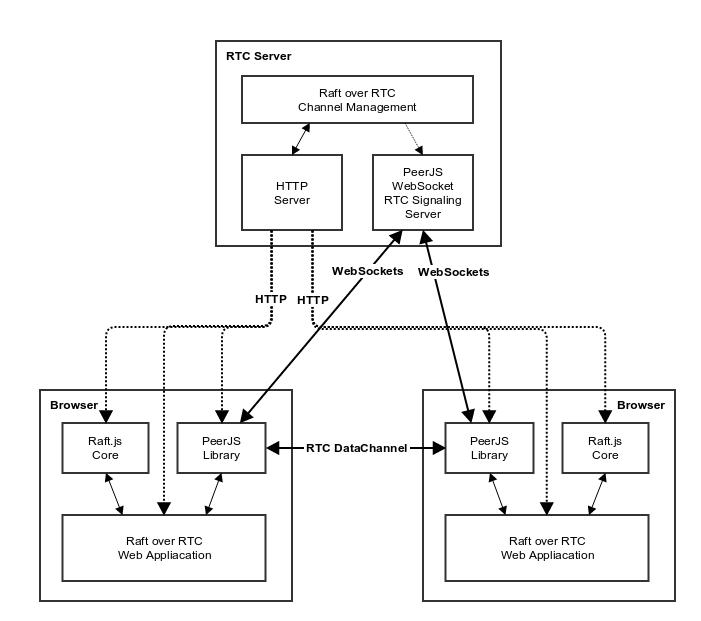
\includegraphics[width=0.45\textwidth]{imgs/raft_rtc_architecture}}
  \caption{Raft over RTC Architecture}
    \label{fig:raft_rtc_architecture}
\end{figure}

\subsection{Raft.js Core Library}

Raft.js is an implementation of the Raft algorithm in JavaScript that
was created by the author of this paper \cite{raft.js}.  Raft.js is
designed to run in either a browser environment or within Node.js
(server-side JavaScript). Raft.js implements the Raft algorithm as
described in \cite[Consensus:~Diego]{raft_thesis:ongaro14}.

\subsubsection{Modular Design}

The implementation of the Raft algorithm is in the
\texttt{RaftServerBase} class (in \texttt{base.js}). The base class
omits the implementation of functions with side-effects such as RPC
communication, durable storage, scheduling/timeouts, or state machine
command/management. In order to create a working implementation these
functions must be provided either as configuration parameters when the
class is instantiated or by sub-classing the class.

The modular design of the Raft.js implementation allows it to be
easily used in different contexts. For example, the \texttt{RaftServerLocal}
class (\texttt{local.js}) implements RPC calls using plain JavaScript function
calls between different instances of the class (nodes) in the same
execution context. For example, the online Raft visualization at
http://kanaka.github.io/raft.js/
%% \href{http://kanaka.github.io/raft.js/}{http://kanaka.github.io/raft.js/}
\cite{raft.js:visualization} uses the \texttt{RaftServerLocal} class
and instantiates it using a scheduling function that executes one
scheduled event each time the user clicks on the ``Step" button rather
than due to the passage of time.

The \texttt{RaftServerHttp} class (\texttt{http.js}) embeds a simple
web server into each Raft node and then uses normal HTTP requests to
send RPC messages between Raft nodes.

For this paper, the \texttt{RaftServerLocal} class was extended with
the capability of sending RPCs over the WebRTC Data Channel.

\subsubsection{Differences between Raft and Raft.js}

The current version of Raft.js implements most of the Raft algorithm
including: leader election, log replication, safety, membership
changes, basic client interaction, and read-only operation
optimizations. % TODO: read-only operations needs mentioning earlier
Log compaction and full client linearizability are not currently
implemented (clients and client transactions are not assigned unique
IDs). Log compaction is important for long-running production systems
in order to limit memory growth and allow new nodes to catch up their
logs more efficiently. However log compaction is not required for
verifying overall system correctness and does not significantly impact
short-running test configurations.

Full client linearizability is an important feature for simplifying
certain types of distributed applications, however the implementation
of linearizability requires some significant additions to the Raft
implementation (e.g. assigning client IDs and sequence IDs and
tracking timed-out clients). For the chat application, simply adding
a single atomic check-and-set state machine command is sufficient to
achieve a linearized chat history.  This does impose a slight
additional cost on the client because it must retry the atomic
operations until they succeed. The author intends to implement both
log compaction and full client linearizability in the future, however
these do not have a significant impact on the ability to test Raft
combined with WebRTC.

The Raft protocol has undergone some revisions since the original
draft paper \cite{raft_paper:ongaro14} (including incorporation of
suggestions by the author of this paper). These changes include
cluster membership simplifications, separating the concepts of
committing entries to the log and applying entries to the state
machine, clearer client interaction, etc. As part of the work for
implementing Raft over WebRTC, the Raft.js implementation was updated
to reflect these changes to the Raft protocol definition.

The are also some other differences between Raft.js and Raft as
described in \cite[Consensus:~Diego]{raft_thesis:ongaro14}:

\begin{enumerate}
\item The paper describes the Raft RPCs in terms of synchronous stream
    based request/response model where requests and responses are
    automatically correlated together by a lower level of the software
    stack. For example with HTTP 1.0 \cite{http:rfc1945} client
    requests are followed by a server response on any given TCP
    stream. Most remote procedure call mechanisms also use
    a synchronous request/response model. %TODO/CITE
    WebRTC DataChannel connections are message based rather than
    request/response stream based. %TODO/CITE
    In the original Raft definition of RPC, request and response messages
    almost contain enough information to function correctly in an
    environment without builtin request/response correlation, such as
    UDP or SCTP when used with reliable transport disabled. %TODO/CITE
    Raft.js includes a small modification to the response RPCs for
    requestVote and appendEntries to add a `sourceId' field that
    enables the protocol to function with message based transports.
\item The Raft paper is clear that each membership change must be
    delayed until all the previous membership change is committed
    (sequential) \cite[Section~4.1]{raft_thesis:ongaro14}. It is
    implied that the leader node should track all pending membership
    change requests and apply them one at a time.  However, in
    Raft.js, if a client requests a membership change while another
    change request is pending (uncommitted), the leader will reject
    the change request with a status of `PENDING\_CONFIG\_CHANGE'.
    This keeps the core Raft implementation simpler with the trade-off
    being that the client implementation of membership change requests
    is slightly more complex due to retry logic.
\end{enumerate}

\ifdefined\OPTIONAL

\subsection{Incremental Steps}

During the planning phase, the project was broken down into ten incremental steps:

\begin{enumerate}
\item Simple WebRTC messaging: implement a small JavaScript
    application that uses the PeerJS client library and an unmodified
    PeerJS signaling server. Demonstrate communication over WebRTC
    DataChannel using two browser instances (or browser tabs).
\item Raft.js over WebRTC: combine the existing Raft.js implementation
    with the small JavaScript application above to demonstrate Raft
    over WebRTC. This step uses a statically configured three node
    cluster (three browser tabs). The PeerJS signaling server is
    polled to retrieve the list of other clients and the Raft cluster
    is started when the number of PeerJS clients reaches three.
\item Update Raft.js protocol: update the Raft.js implementation to
    match the latest description of the Raft protocol
    \cite{raft_thesis:ongaro14}. This includes the implementation of
    the simplified membership change algorithm (sequential changes)
    and the separation of the log commit and state machine apply
    concepts.  Additionally, the new Raft.js implementation always
    starts a new Raft cluster as a cluster with a single node and
    additional nodes are dynamically added to the cluster
    \cite[Section~4.4]{raft_thesis:ongaro14}.
\item Dynamic Raft.js over WebRTC: enhance the signaling server with
    support for multiple sessions/channels to enable separate Raft
    clusters with the same signaling server. Start each cluster with
    a single node and automatically add and remove Raft nodes as they
    come and go.
\item Visual representation: display Raft node state and RPC
    statistics in addition to the internal Raft logging messages.
\item Sessionless/Datagram RPC messages: change Raft RPC requests and
    response messages so that RPC responses have enough context to be
    handled separately from RPC requests. Specifically this enables
    Raft to support datagram (sessionless) network transports like
    WebRTC.
\item Atomic state machine operation: implement a state machine
    update operation that only succeeds if no other operation has been
    applied to the same key since the last time this client read from
    that key.
\item Automatic client request forwarding: extend the client request
    RPC to also be sessionless/datagram based. Implement an
    asynchronous JavaScript function that determines which node is the
    leader and forwards client request RPCs to the leader. This
    function must also correlate RPC responses to the client request
    and invoke the callback for the original request.
\item Chat application: add the ability to send a chat message to the
    log using the client request forwarding functionality together
    with atomic state machine operation. Show the current chat history
    based on the chat entries in the state machine.
\item Server as Raft.js peer (aspirational): enable server nodes
    (Raft.js running on Node.js) to fully participate as Raft cluster
    nodes.
\end{enumerate}

Steps 1-9 were successfully implemented for this paper. Step 10 was an
aspirational goal because this functionality is not yet supported in
PeerJS \cite{peerjs:103}.

\fi  % \ifdefined\OPTIONAL

\subsection{Server}

The file `rtc\_server.js' implements the signaling server for the Raft
over WebRTC application. The server extends the PeerJS
`ExpressPeerServer' object in order to provide WebRTC signaling. In
addition to the WebRTC signaling function the server also provides the
following service endpoints:

\begin{enumerate}
\item Static web service endpoint: this serves the static HTML, CSS
    and JavaScript that make up the Raft over WebRTC web application.
\item New channel endpoint: when a browser loads this endpoint, a new
    PeerJS channel is created and the browser is redirected to a URL
    for loading the main application (via static file service above).
    The redirect URL has a query string appended that contains the
    channel ID of the new channel that was just created. In addition
    the redirect URL has a fragment identifier (hash/history) that
    communicates to the web application that this is the first server
    in the channel.
\item Peer list endpoint: this endpoint takes a channel ID and returns
    the list of WebRTC peers (browser user agents) that are currently
    connected to that channel.

\end{enumerate}

Refer to Section~\ref{section:design-client} and
Figure~\ref{fig:raft_rtc_sequence} for a description of how these
endpoints interact.

\subsection{Client}
    \label{section:design-client}

The Raft over WebRTC testing application is designed as a single web
page (\texttt{rtc.html} or \texttt{chat.html}). The application has
different starting behavior depending on the value of the URL query
string (the URL component following the ``?" and up to the ``\#") and
the fragment identifier (the URL component after the ``\#").

When a new Raft cluster is created, the user agent (browser) connects
to the server's new channel endpoint
(Figure~\ref{fig:raft_rtc_sequence}~[1]). This endpoint causes the
server to create a new channel for PeerJS signaling
(Figure~\ref{fig:raft_rtc_sequence}~[2]). Once this is complete the
server responds to the browser with a redirect message
that contains the new channel identifier in the query parameter and an
indication that this is the very first Raft cluster node in the
fragment identifier (Figure~\ref{fig:raft_rtc_sequence}~[3]).

The browser follows the redirect and loads the static web application
at the static file endpoint provided by the server
(Figure~\ref{fig:raft_rtc_sequence}~[4]). This includes the
main application page (\texttt{rtc.html} or \texttt{chat.html}), the
core raft algorithm (\texttt{base.js} and \texttt{local.js}), the
PeerJS client library (\texttt{peer.js}), the actual Raft over WebRTC
implementation (\texttt{rtc.js}), a layout stylesheet
(\texttt{web/demo.css}), and higher-level application code if that is
being loaded (\texttt{chat.js})
(Figure~\ref{fig:raft_rtc_sequence}~[5]).

If the URL fragment identifier is set to ``firstServer", then this Raft
node is initialized as the leader of a single node cluster and all
normal timers are started. The fragment identifier is then unset. The
query parameter contains the ID of this cluster (the PeerJS channel).

Subsequent nodes are added to the same Raft cluster by starting a new
browser context (separate browser, browser window, or browser tab) and
loading the same URL without the ``firstServer" fragment identifier
(Figure~\ref{fig:raft_rtc_sequence}~[9]). There is a convenience link
provided in the application page that opens a new browser window with
a new cluster node.  %(see \ref{fig:browser_1}).

When each page first loads, a PeerJS signaling connection is
established with the server
(Figure~\ref{fig:raft_rtc_sequence}~[6]~and~[11]). Once this
connection is established, the application will be notified when any
PeerJS clients connect to or disconnect from the server.  After the
PeerJS signaling connection is established, the client immediately
queries the Peer list endpoint
(Figure~\ref{fig:raft_rtc_sequence}~[7]~and~[12]~and~[14]]) to discover
any clients that were connected prior to when this node connected to
the server (Figure~\ref{fig:raft_rtc_sequence}~[8]~and~[13]~and~[15]]).

The web application also begins a periodic async polling function
(\texttt{addRemoveServersAsync}) when the page loads. When the node is a Raft
leader, the function compares the current active list of PeerJS clients to
the Raft cluster membership list. If there are any differences between
the two lists, then any new clients are added to the Raft cluster and
missing clients are removed from the Raft cluster one at a time using
the \texttt{addServer} and \texttt{removeServer} RPC calls. Servers
additions are prioritized before removals 
in order to maximize availability
\cite[Section~4.4]{raft_thesis:ongaro14}.

When an instance of the web application starts that is not
a ``firstServer", the normal Raft timers are not enabled until the
server receives its first RPC. The prevents the server from
trying to becoming a leader before it is incorporated into the cluster
by an appendEntries RPC from the true cluster leader.

\subsubsection{Client Statistics}

In addition to the low level Raft message log, the following
statistics are shown in the application:
\ifdefined\OPTIONAL

\begin{enumerate}
\item \emph{Term}: the current Raft leadership term.
\item \emph{State}: the current Raft node state (follower, candidate,
    or leader)
\item \emph{Cluster Size}: a count of the current Raft cluster
    membership (number of nodes currently participating in the
    cluster)
\item \emph{Log Length}: number of entries in the transaction log.
\item \emph{Request Votes Sent/Received}: the number of `requestVote`
    RPCs that have been sent from and received by this node.
\item \emph{Append Entries Sent/Received}: the number of
    `appendEntries' RPCs that have been sent from and received by this
    node.
\end{enumerate}
\else
the current Raft leadership term, the current Raft node state
(follower, candidate, or leader), Raft cluster size (number of
participating nodes), number of entries in the transaction log, and
number of request vote and append entries RPCs that have been sent and
received.
\fi

\subsubsection{Client Request Redirects}

% TODO: rename clientRequest* function to not clash with RPC names
% (maybe raftRequest*?)

In the Raft over WebRTC implementation each local browser is a client
of the Raft cluster. However in Raft, the leader node is the only node
that adds entries to the log so clients on follower nodes must have
a way to communicate with the leader.
\ifdefined\OPTIONAL
This is implemented as a pair of
functions named \texttt{clientRequest} and
\texttt{clientRequestResponse}. The \texttt{clientRequest} function is
called by the client with the arguments of a client request RPC and
a callback function to be called once the request is completed. The
\texttt{clientRequest}/\texttt{clientRequestResponse} functions work
as follows:

\begin{enumerate}
\item The \texttt{clientRequestResponse} is registered with the local
    Raft.js implementation as the callback function anytime
    a \texttt{clientRequestResponse} RPC is received.
\item The \texttt{clientRequest} function keeps track of the current
    leader ID.  If the current leader ID is not set or this node is
    the leader then the client request RPC is sent directly to the
    local Raft node bypassing the network transport layer.  If the
    current leader ID is set then the request is sent to that node as
    a normal RPC request over the WebRTC channel.
\item When the \texttt{clientRequestResponse} function is called and
    the status is ``NOT\_LEADER" then the current leader ID being
    tracked by the \texttt{clientRequest} function is set to the
    leader ID specified in the response. Then the original request is
    re-issued over the normal WebRTC channel to the leader.
\item When the \texttt{clientRequestResponse} function is called with
    a successful status, the original callback argument of the
    \texttt{clientRequest} function is called with the results from
    the RPC response.
\end{enumerate}
\else
When a \texttt{clientRequest} message is sent to a local Raft node
that is not the leader, the \texttt{clientRequestResponse} message
will be returned with a status of ``NOT\_LEADER" and the ID of the
current leader. The \texttt{clientRequest} message will then be
re-issued over the WebRTC DataCannel to the leader ID that was
returned.
\fi

\subsection{Chat Application}

\begin{figure}[!t]
  \centerline{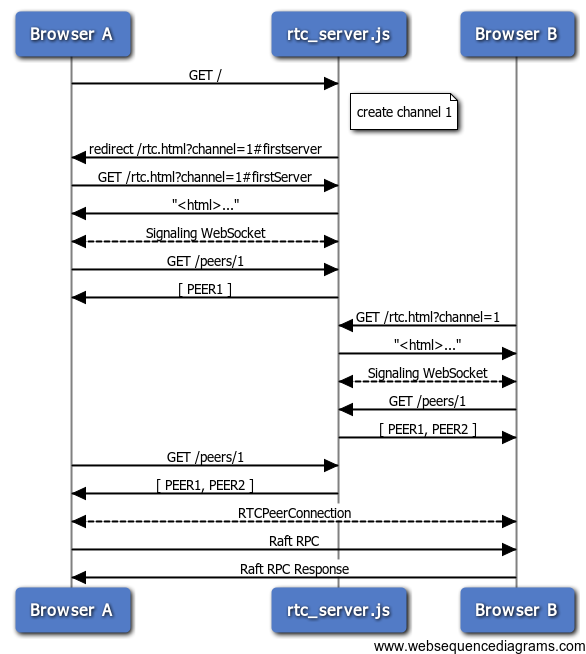
\includegraphics[width=0.45\textwidth]{imgs/raft_rtc_sequence}}
  \caption{Raft over RTC Sequence Diagram}
    \label{fig:raft_rtc_sequence}
\end{figure}

The chat application extends the basic Raft.js over WebRTC client. The
chat application provides a large text area containing the chat
history and a text entry field below it. % (see Figure~\ref{fig:browser_chat_1}).
When the user clicks on the \emph{Send} button (or presses enter), the
current node ID is prepended to the beginning of the text line and it
is added to a pending send queue and the text entry field is blanked.
\ifdefined\OPTIONAL
A function to flush the send queue runs periodically (currently every
100ms) and does the following:
% TODO: 100ms above should be less

\begin{enumerate}
\item If there is line of text that has been sent but not yet
    added (applied) to the state machine or there are no lines of text
    on the pending send queue, then the function does nothing.
\item A text line is removed from the head of the pending send queue
    and stored in \emph{curSend} to indicate that a send is in
    progress. Then a client request is made using an atomic
    \emph{seqAppend} command to add the new text to the state machine
    (\emph{seqAppend} is described below).  The \emph{seqAppend}
    operation attempts to append the text line to a list at the
    \emph{history} key in the state machine.
\item When the atomic \emph{seqAppend} operation completes, it may
    have failed (if another text line was appended first), in which
    case the flush function puts the failed text line back on the
    pending send queue. Whether the send was successful or failed, the
    \emph{curSend} variable is set to nil/null to indicate that no
    send is in progress. The next time the flush function runs it will
    attempt to send again. % TODO: reword
\end{enumerate}
\else
A function to flush the send queue runs periodically (currently every
100ms) to send the chat message at the head of the queue using
the \emph{seqAppend} operation.
\fi

% TODO: normalize use of \texttt and \emph

The chat application extends the default set of state machine
operations to add the \emph{seqAppend} operation. This is an atomic
operation that is implemented as follows:

\begin{enumerate}
\item The \emph{seqAppend} operation operates on a specially
    structured key/value pair in the state machine map. The value of
    the pair is another associative map that contains a counter and
    list structure where the actual chat lines are accumulated.
    \emph{seqAppend} operations are sent with both a count and the new
    value to append.
\item When a \emph{seqAppend} operation is applied to the state
    machine and the count value in the command matches the counter in
    the state machine's value, then the new line in the request is
    added to the value list and the counter is incremented. If the
    count value does not match the counter then the the operation is
    not applied. In either case, a list is returned in the
    \texttt{clientRequestResponse} that contains two values: a Boolean
    indicating whether the \emph{seqAppend} operation succeeded and
    a number indicating the current value of the counter.
\item The first time the \emph{seqAppend} operation is used on
    a non-existent key, the structure previously described is created
    with the counter set to 0 and the list structure is created with
    the single value that was passed in the \emph{seqAppend}
    operation.
\item Clients that call the \emph{seqAppend} operation should check
    the status value in the result list. If the status is false, then
    the client should retry the operation. Regardless of success of
    failure, then client should store the current value of the counter
    for the next \emph{seqAppend} call or retry.
\end{enumerate}

\section{Experimental Results}


\ifdefined\OPTIONAL

\subsection{Manual Testing}

\subsubsection{Setup}

The initial way that the application was tested was by loading the
basic application to create a Raft over WebRTC cluster with a single
node acting as leader. Figure~\ref{fig:browser_1} shows a screenshot
of the browser after the first node is created:

\begin{figure}[!t]
    \centering
    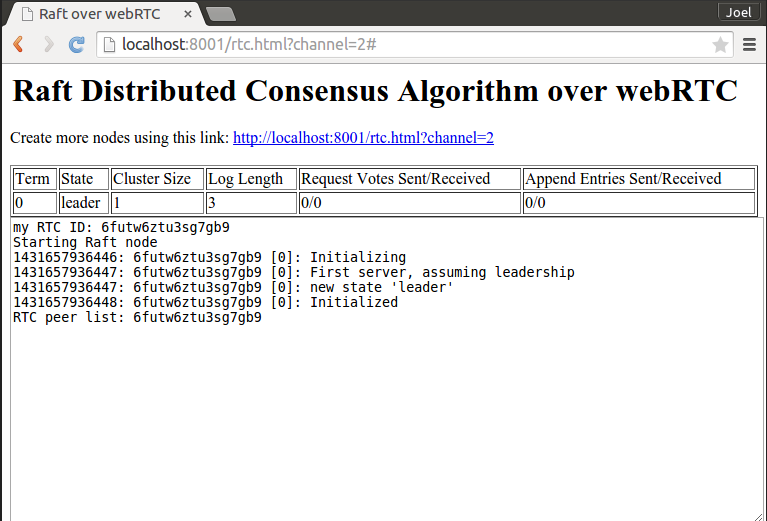
\includegraphics[width=0.45\textwidth]{imgs/browser_1.png}
    %\captionof{figure}{Basic app with one Node/Tab}
    \caption{Basic app with one Node/Tab}
    \label{fig:browser_1}
\end{figure}

Then four more Raft nodes were then added to the cluster by clicking
on the embedded ``create more nodes" link in the application.
Figure~\ref{fig:browser_5} shows a screenshot of the browser once four
new nodes are added to the cluster (5 total):

\begin{figure}[!t]
    \centering
    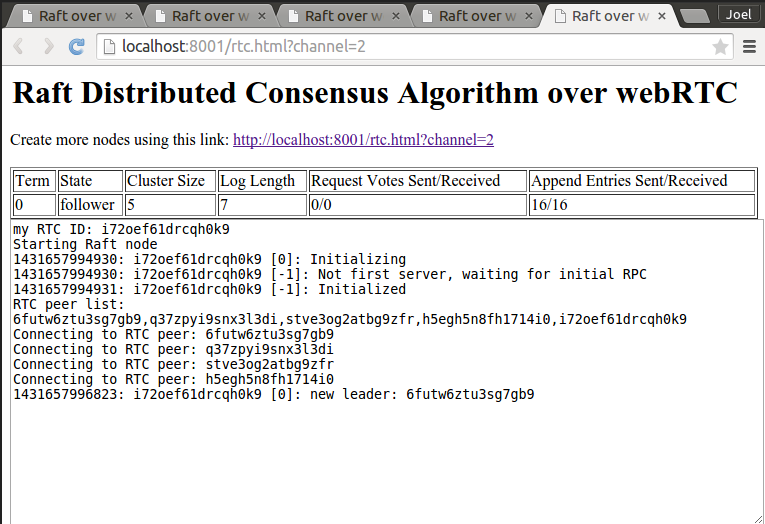
\includegraphics[width=0.45\textwidth]{imgs/browser_5.png}
    %\captionof{figure}{Basic app with Five Nodes/Tabs}
    \caption{Basic app with Five Nodes/Tabs}
    \label{fig:browser_5}
\end{figure}

In addition, the full chat application was also tested manually by
loading the initial chat application landing page to create a Raft
over WebRTC cluster with a single node acting as leader. Then lines
of text were entered into the text area each followed by clicking the
Send button. Figure~\ref{fig:browser_chat_1} shows a screenshot of the
browser after the first node/tab of the chat application is created
and a line of text was sent:

\begin{figure}[!t]
    \centering
    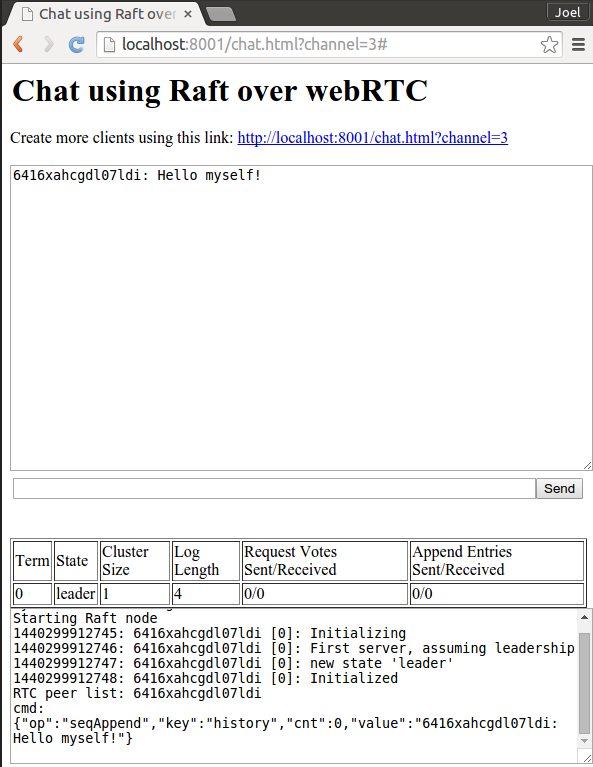
\includegraphics[width=0.45\textwidth]{imgs/chat_1a.png}
    %\captionof{figure}{Chat app with one Node/Tab}
    \caption{Chat app with one Node/Tab}
    \label{fig:browser_chat_1}
\end{figure}

Then four more Raft nodes were then added to the cluster by clicking
on the embedded ``create more clients" link in the application.
Finally, on a non-leader node more text lines were entered and sent by
clicking the Send button. Figure~\ref{fig:browser_chat_5} shows
a screenshot of the browser once four new nodes/tabs are added to the
cluster (5 total) and another text line was sent from the fifth node:

\begin{figure}[!t]
    \centering
    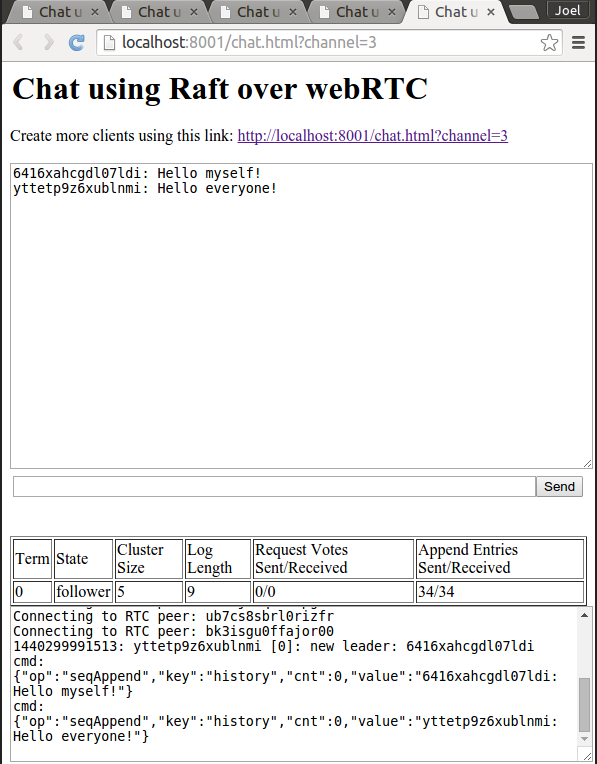
\includegraphics[width=0.45\textwidth]{imgs/chat_5a.png}
    %\captionof{figure}{Chat app with Five Nodes/Tabs}
    \caption{Chat app with Five Nodes/Tabs}
    \label{fig:browser_chat_5}
\end{figure}

After every change was made to the cluster all the nodes were checked
to ensure that the following steady state properties were observed:
\begin{enumerate}
\item only a single leader
\item all nodes have the same term and transaction log count
\item all non-leader nodes are receiving `appendEntries' RPCs from the leader
\item all nodes have the same cluster membership state
\item the transaction log entries are identical on all nodes
\item the state machine is identical on all nodes
\end{enumerate}

The current leader was then terminated. The other nodes were checked
again the steady state properties. This was repeated until only two
nodes remained in the cluster.

Next the five node cluster was brought up again and state machine
commands were sent to leader to add to the transaction log. Again the
nodes were checked for the above steady state properties.

Then the application was tested by loading the initial cluster
creation landing page in a browser tab. Nodes were randomly added to
the cluster (by clicking on the link embedded in the page) or removed
from the cluster (by closing a tab). After each change the steady
state properties were checked.

Similar testing to the above was done with browser instances on two
separate computers. In addition, cross-browser functionality was
verified by running nodes from the same cluster running simultaneously
in Chrome 42 and Firefox 37.


\subsubsection{Outcome}

The results of the manual testing above showed that Raft over WebRTC
was able to perform leader elections correctly, the log and state
machine were replicated correctly to all nodes, and the safety
properties were maintained. During testing the membership of the
cluster was changed numerous times (both node additions and removals)
and the Raft properties were maintained throughout. In addition,
client interaction was tested to make sure commands were still
properly added to the state machine and transaction log.

One limitation of the Raft protocol is that if the cluster membership drops from
two nodes to one node, then the cluster will become unavailable without manual
intervention. This is because both nodes of a two-node cluster are required for
a majority vote.  When one member of a two-node cluster is forcibly shut down,
then the remaining cluster node will be unable to win elections or even commit
transaction entries, and the cluster will become unavailable. There are several
options to get around this problem:

% NOTE: optional section

\begin{enumerate}
\item The node can ask the leader to be removed and then wait for the
  transaction to become effective before it disconnects.  This may not
  always be an option especially in a browser context where the user
  may immediately kill the window/tab without giving the application
  a chance to remove itself from the cluster.
\item The signaling server can serve as a tie-breaker. This would allow
  the remaining leader successfully commit the removal of the other
  node. In the case of a partition, the signaling server must only
  vote for one of the nodes.
\item The node with the lower ID could have an implicit tie-breaker vote.
  This would allow one node of the partition to continue in the case
  of a network partition. If a node dies or is killed, this would only
  allow the cluster to continue to operate if the node that survives
  happens to have the lower ID.
\item The system could allow manual user intervention. However, this is
  only likely to work correctly in the case where the user of the last
  remaining node can be certain that other nodes will never return;
  otherwise there is a risk of data-corruption.
\end{enumerate}

Running a Raft cluster in a browser context can lead to some level of
timer instability. The JavaScript execution context is a fully event
driven environment with a single thread of execution for a given
JavaScript context. JavaScript code is run when browser (or Node.js)
events trigger JavaScript code that is registered to that event. In
order to implement logic that runs periodically, JavaScript code is
registered as a callback timer using the setTimer, setInterval or
requestAnimationFrame APIs. However, none of these mechanisms is
a precise timer. When a timer fires, the callback code it refers to
is added to the JavaScript execution queue and events on the queue are
processed in the order they arrive. This means callbacks may be
delayed by other code that is already running or queued first
\cite{resig2013secrets}.

However, there is another browser mechanism that is less well known
but that causes even larger delays in timer code execution. Modern
browsers often have dozens or even hundreds of windows and/or tabs
open simultaneously. In order to reduce CPU load, increase user
responsiveness and improve battery life, most modern browsers will
throttle the JavaScript callback timers for all windows and tabs that
are hidden or have not been directly interacted with for some period
of time. This throttling can cause timers to slow down by an order of
magnitude or more. %TODO/CITE

In the context of Raft over WebRTC, the slowdown of background page
timers means that whenever the leader node is residing on a page that
is in the background, the propagation of transaction log entries slows
down substantially. This also means that other nodes which are in the
foreground are more likely to have an election timeout timer fire and
they are more likely to become a leader because they will be able to
send and receive votes more quickly than nodes that are in the
background.  In this sense the problem is self-correcting over
the long term because higher performing nodes more are likely to start
and win elections. This also indicates that dynamic adjustment of timeout
values may be a fruitful area of further study.

In the context of the full chat application the slowdown of background
pages is even more pronounced because each addition to the chat
history can take several messages to fully propagate the new date. An
interesting area of further study would be to extend the Raft protocol
to more proactively adapt to network and node performance conditions
(delayed timers) and more intentionally transition leadership to more
capable nodes.

\fi  % \ifdefined\OPTIONAL


\subsection{Automated Testing}

\subsubsection{Twst Test Framework}

In order to facilitate coordinated testing across a large number of
browser instances, a new test framework was created called
\cite{twst}. This \emph{Twst} framework provides a client and server
library written in JavaScript:

\begin{enumerate}
    \item \emph{server library}: this library is used to write tests
        that need to coordinate testing across many browser instances.
        It provides services such as client tracking/enumeration,
        broadcast and targeted RPC, state rendezvous, log collection,
        etc.
    \item \emph{client library}: this library is included with the web
        application that is being tested. When the page loads, the
        library will automatically connect to the \emph{Twst} server
        instance and begin sending console logs and accepting
        RPCs/commands from the server.
\end{enumerate}


\subsubsection{Test Setup}

Automated testing of the Raft over WebRTC system was performed by
leveraging the SlimerJS scriptable browser environment. SlimerJS
enables web applications to be scripted by loading pages in a special
Mozilla rendering environment called XULRunner. The XULRunner instance
is directed to an X virtual frame buffer (xvfb) which provides
effectively headless testing.

To simplify the execution of the tests and to make the testing
infrastructure more portable, a docker container environment
encapsulates and executes the SlimerJS environment. The container is
built using \emph{test/Dockerfile} which is in turn derived from the
``fentas/slimerjs" docker image \cite{fentas:slimerjs}.
This custom Dockerfile was created because the upstream version of the
Dockerfile used an older version of XULRunner that did not support
more than 7 WebRTC clients communicating together simultaneously. This
issue was discovered during initial testing.

Writing tests using SlimerJS involves creating JavaScript test
programs which start a \emph{Twst} server instance and then launch a SlimerJS
docker container for each node of the cluster. Each container starts
a XULRunner browser instance of the Raft over WebRTC chat application.
Also included with the application is the \emph{Twst} client library
which connects back to the \emph{Twst} service in the test program.
Once all the chat application nodes have connected to the test
server/program, then the actual test is started across all the
application nodes.

Three different tests programs/servers were created to test the basic
Raft over WebRTC application. Each of the tests takes a parameter
indicating the number of nodes/pages to launch. The test source files
are:

\begin{enumerate}
    \item \emph{test/common.js}: a module of common functions used by
        the other tests scripts.
    \item \emph{test/test\_up.js}: launch and start an initial leader
        node/page, then start the rest of the nodes (if any) so that
        the leader will configure them into the cluster. Then test
        then waits for every node to be recorded (applied) into the
        log of every other node of the cluster. The test reports the
        number of milliseconds for the cluster to reach this state.
    \item \emph{test/test\_kill\_nodes.js}: similar to
        \emph{test/test\_up.js} but once all the nodes are configured
        into the cluster, this script then kills the leader plus
        a configurable number of nodes. By default the script kills
        just under half the nodes of the cluster. The test then waits
        for a new leader to be elected and remove the dead nodes from
        the cluster. The test reports both the number of milliseconds
        for the cluster to come up and the number of milliseconds for
        the cluster to fully recover from the failure and evict the
        failed nodes.
    \item \emph{test/test\_chat\_propagate.js}: similar to
        \emph{test/test\_up.js} but once the cluster is up, the test
        connects to one of the non-leader nodes and and sends a chat
        text line. The test then waits for the chat message to
        propagate to every other node's state machine. The test
        reports both the number of milliseconds for the cluster to
        come up and for the messages to propagate to every node.
\end{enumerate}

\ifdefined\OPTIONAL
The tests were all run on a system with the following configuration:

\begin{enumerate}
    \item \emph{CPUs}: 8 Intel Core i7 processors running at 3.20GHz
    \item \emph{Memory}: 12 GB
    \item \emph{OS}: Ubuntu 14.04.1 LTS
    \item \emph{Docker}: version 1.3.1
    \item \emph{Docker image}:
    \begin{enumerate}
        \item \emph{OS}: Ubuntu 12.04.5 LTS
        \item \emph{SlimerJS}: version 0.9.6
        \item \emph{XULRunner}: 38.0.5
    \end{enumerate}
\end{enumerate}
\else
The tests were all run on a system with 8 Intel Core i7 processors
running at 3.20GHz and 12 GB of main memory. The Docker image used to
run the test was built using Ubuntu 12.04.5 LTS with \emph{SlimerJS}
version 0.9.6, and \emph{XULRunner} version 38.0.5.
\fi


Five different tests (using different options for the three test
programs) were run at 17 different cluster sizes (odd cluster sizes
from 3 to 35 nodes). Each of these tests was run with three different
Raft election timeout values: 250ms, 500ms, 1000ms. Each of the five
tests and cluster size combinations was run 7 times.

\subsubsection{Outcome}

\begin{figure}[!t]
    \begin{tikzpicture}
    \begin{axis}[%
        xlabel={Nodes}, ylabel={Time (seconds)},
        %xtick=data,
        xmin=0, ymin=0,
        grid=major,
        scatter/classes={%
            propagate_1_et1000={mark=x,draw=blue},
            propagate_1_et1000_average={mark=}}]
    \addplot[scatter,only marks,%
        scatter src=explicit symbolic]%
    table[meta=label] {data/propagate_1.dat};
    \addplot[scatter,%
        scatter src=explicit symbolic]%
    table[meta=label] {data/propagate_1_average.dat};
    \end{axis}
    \end{tikzpicture}
    \caption{Propagate$,$ Commit$,$ and Apply 1 Command}
    \label{fig:propagate1}
%
    \vspace{1cm}
%
    \begin{tikzpicture}
    \begin{axis}[%
        xlabel={Nodes}, ylabel={Time (seconds)},
        %xtick=data,
        xmin=0, ymin=0,
        grid=major,
        scatter/classes={%
            propagate_100_et1000={mark=x,draw=blue},
            propagate_100_et1000_average={mark=}}]
    \addplot[scatter,only marks,%
        scatter src=explicit symbolic]%
    table[meta=label] {data/propagate_100.dat};
    \addplot[scatter,%
        scatter src=explicit symbolic]%
    table[meta=label] {data/propagate_100_average.dat};
    \end{axis}
    \end{tikzpicture}
    \caption{Propagate$,$ Commit$,$ and Apply 100 Commands}
    \label{fig:propagate100}
\end{figure}

\begin{figure}[!t]
    \begin{tikzpicture}
    \begin{axis}[%
        %height=1.5\textwidth, width=1.4\textwidth,
        %width=0.45\textwidth,
        xlabel={Nodes}, ylabel={Time (seconds)},
        xmin=0, xmax=37,
        ymin=0, ymax=15,
        grid=major,
        %legend pos=outer north east,
        legend pos=north west,
        scatter/classes={%
            start_et1000={mark=x,draw=blue},
            start_et1000_average={mark=,draw=red},
            start_et500={mark=x,draw=cyan},
            %start_et500_fail={mark=x,draw=red},
            start_et500_average={mark=,draw=red},
            start_et250={mark=x,draw=magenta},
            %start_et250_fail={mark=x,/raw=red}
            start_et250_average={mark=,draw=red}}]
    \addplot[scatter,only marks,%
        scatter src=explicit symbolic]%
    table[meta=label] {data/start_et1000.dat};
    \addplot[blue,scatter,%
        scatter src=explicit symbolic]%
    table[meta=label] {data/start_et1000_average.dat};

    \addplot[scatter,only marks,%
        scatter src=explicit symbolic]%
    table[meta=label] {data/start_et500.dat};
    %\addplot[scatter,%
    %    scatter src=explicit symbolic]%
    %table[meta=label] {data/start_et500_fail.dat};
    \addplot[cyan,scatter,%
        scatter src=explicit symbolic]%
    table[meta=label] {data/start_et500_average.dat};

    \addplot[scatter,only marks,%
        scatter src=explicit symbolic]%
    table[meta=label] {data/start_et250.dat};
    \addplot[magenta,scatter,%
        scatter src=explicit symbolic]%
    table[meta=label] {data/start_et250_average.dat};

    \legend{1000ms,,500ms,,250ms,}
    \end{axis}
    \end{tikzpicture}
    \caption{Initial Cluster Activation}
    \label{fig:cluster_up}
\end{figure}

\begin{figure}[!t]
    \begin{tikzpicture}
    \begin{axis}[%
        %height=1.5\textwidth, width=1.4\textwidth,
        %width=0.45\textwidth,
        xlabel={Nodes}, ylabel={Time (seconds)},
        xmin=0, xmax=37,
        ymin=0, ymax=4.5,
        grid=major,
        %legend pos=outer north east,
        legend pos=north west,
        scatter/classes={%
            kill_1_et1000={mark=x,draw=blue},
            kill_1_et1000_average={mark=,draw=red},
            kill_1_et500={mark=x,draw=cyan},
            %kill_1_et500_fail={mark=x,draw=red},
            kill_1_et500_average={mark=,draw=red},
            kill_1_et250={mark=x,draw=magenta},
            %kill_1_et250_fail={mark=x,/raw=red},
            kill_1_et250_average={mark=,draw=red}}]
    \addplot[scatter,only marks,%
        scatter src=explicit symbolic]%
    table[meta=label] {data/kill_1_et1000.dat};
    \addplot[blue,scatter,%
        scatter src=explicit symbolic]%
    table[meta=label] {data/kill_1_et1000_average.dat};

    \addplot[scatter,only marks,%
        scatter src=explicit symbolic]%
    table[meta=label] {data/kill_1_et500.dat};
    %\addplot[scatter,%
    %    scatter src=explicit symbolic]%
    %table[meta=label] {data/kill_1_et500_fail.dat};
    \addplot[cyan,scatter,%
        scatter src=explicit symbolic]%
    table[meta=label] {data/kill_1_et500_average.dat};

    \addplot[scatter,only marks,%
        scatter src=explicit symbolic]%
    table[meta=label] {data/kill_1_et250.dat};
    \addplot[magenta,scatter,%
        scatter src=explicit symbolic]%
    table[meta=label] {data/kill_1_et250_average.dat};

    \legend{1000ms,,500ms,,250ms,}

    \end{axis}
    \end{tikzpicture}
    \caption{Recovery from Leader Failure}
    \label{fig:recovery_leader_failure}
%
    \vspace{1cm}
%
    \begin{tikzpicture}
    \begin{axis}[%
        %height=1.5\textwidth, width=1.4\textwidth,
        %width=0.45\textwidth,
        xlabel={Nodes}, ylabel={Time (seconds)},
        xmin=0, xmax=37,
        ymin=0, ymax=4.5,
        grid=major,
        %legend pos=outer north east,
        legend pos=north west,
        scatter/classes={%
            kill_half_et250={mark=x,draw=magenta},
            kill_half_et250_average={mark=,draw=red},
            %kill_half_et250_fail={mark=x,/raw=red},
            kill_half_et500={mark=x,draw=cyan},
            kill_half_et500_average={mark=,draw=red},
            %kill_half_et500_fail={mark=x,draw=red},
            kill_half_et1000={mark=x,draw=blue},
            kill_half_et1000_average={mark=,draw=red}}]
    \addplot[scatter,only marks,%
        scatter src=explicit symbolic]%
    table[meta=label] {data/kill_half_et1000.dat};
    \addplot[blue,scatter,%
        scatter src=explicit symbolic]%
    table[meta=label] {data/kill_half_et1000_average.dat};

    \addplot[scatter,only marks,%
        scatter src=explicit symbolic]%
    table[meta=label] {data/kill_half_et500.dat};
    %\addplot[scatter,%
    %    scatter src=explicit symbolic]%
    %table[meta=label] {data/kill_half_et500_fail.dat};
    \addplot[cyan,scatter,%
        scatter src=explicit symbolic]%
    table[meta=label] {data/kill_half_et500_average.dat};

    \addplot[scatter,only marks,%
        scatter src=explicit symbolic]%
    table[meta=label] {data/kill_half_et250.dat};
    \addplot[magenta,scatter,%
        scatter src=explicit symbolic]%
    table[meta=label] {data/kill_half_et250_average.dat};

    \legend{1000ms,,500ms,,250ms,}

    \end{axis}
    \end{tikzpicture}
    \caption{Recovery from Half Cluster Failure}
    \label{fig:recovery_half_failure}
\end{figure}



Figure~\ref{fig:propagate1} and Figure~\ref{fig:propagate100} show the
result of running the \emph{test/wait\_chat\_propagate.js} test to
determine the amount of time that a stable cluster takes to propagate,
commit and apply 1 and 100 chat message commands respectively to the state
machine on every cluster node using the atomic \emph{seqAppend}
command. The commands are serialized which means that the previous
command must be committed before the current command can be committed.
The test is complete once the last chat message command has been both
committed and applied to every node of the cluster. Each test execution
is shown as a blue ``x" and the black line represents the average for
each cluster size.

In Figure~\ref{fig:propagate1} the time to propagate a single message
to a single node of the cluster is approximately 0.1 seconds. This
simply represents the tests scanning/checking granularity.  The time
to finish propagating and committing a single message shows a slight
linear slope upwards from about 0.3 seconds for a three node cluster
to about 0.5 seconds for a 41 node cluster. The time to propagate 100
messages (Figure~\ref{fig:propagate100}) has a much higher slope and
also appears to be non-linear. % TODO: why?

Figure~\ref{fig:cluster_up} shows the results of running the
\emph{test/test\_up.js} test to determine the amount of time that
a cluster takes to start. The cluster is fully started once a leader
has been elected and the leader has successfully added all the other
nodes to the running configuration. Each election timer value is
represented as a different color and the line represents the average
value for each cluster size. The cluster startup times show a fairly
linear increase as the cluster size increases. The reason that the
slope varies with election timer is due to the fact that the election
timer also determines the leader heartbeat value (currently set to one
fifth of the election timer value). The leader heartbeat determines
the frequency with which \emph{appendEntries} messages are sent from
the leader to followers and is also used to propagate log entries.
This means that the rate at which log entries (and thus cluster
configuration updates) can be propagated is proportional to the
election timer value.

Figures \ref{fig:recovery_leader_failure} and
\ref{fig:recovery_half_failure} show the results of running the
\emph{test/test\_kill\_nodes.js} in both modes (kill only leader and
kill just under half the nodes). Each election timer value is
represented as a different color and the solid line represents the
average recovery time for each cluster size. When only the leader is
killed, the recovery times are constant flat regardless of cluster
size. This is because after a new leader is elected, there is only
a single configuration entry to propagate to the rest of the cluster
(to remove the old failed leader). One interesting thing to note is
that with a 1000ms timer, the 3 node cluster is actually the most
inefficient size because the average time until a leader election
starts is inversely proportional to cluster size so the delay until an
election happens is a significant contributor to the three node
cluster with 1000ms timer. With a larger cluster or shorter election
timer, the contribution of election delay is not noticeable. The
recovery from almost half the nodes failing is not flat because the
amount of configuration information that needs to be propagated is
proportional to the size of the cluster.

At larger cluster sizes (35 and greater) the cluster begins to
experience failures. For example, when testing with a 250ms election
timer, once the cluster size reaches 35 nodes, the cluster is
frequently (more than 50\% of the time) unable to recover from the
half cluster shutdown test. At a cluster size or 41 and with a 1000ms
election timer, the cluster begins to experience difficulty
successfully starting up (about 50\% failure rate). The basic problem
appears to be due to the average election timeout period being too low
in relation to communication latency. During leader election, the
first candidate is unable to gather enough votes to become leader
before other candidates arise and steal votes which prevents a quorum.

Some (or most) of the communication latency may be a result of CPU or
memory contention due to all the browser instances running on a single
host. The use of multiple hosts may show that the system can support
much larger clusters for a given election timeout value. However, with
a fixed election timer value, there is always a cluster size for which
communication latency will begin to prevent the cluster from being
able to perform leader elections. A dynamically adjusted election
timer is something that should be explored especially for a browser
context where the communication latency may be highly variable over
time.


\section{Future Work}

One of the useful outcomes of this project was that it brought to
light many areas where further study of Raft, WebRTC, and Raft over
WebRTC should be pursued. Here are some interesting areas for further
exploration:

\begin{enumerate}
\item Explore models for dynamically adjusting Raft timeout values to
    account for changing network and browser conditions.
\item Explore alternate WebRTC transport modes for relaxing ordering
    constraints and delivery guarantees. Since the Raft protocol is
    tolerant of out-of-order and dropped messages, it is possible that
    Raft over WebRTC could be more efficient with one or both of these
    constraints relaxed.
\item Test the survivability of the cluster when the signaling server
    becomes completely unresponsive or very slow.
\item Test larger scale deployments spanning larger and more diverse
    network domains. Characterize the factors that affect and limit
    scalability.
\item Explore models for dealing with the case where the cluster goes
    from two nodes down to one node. Can usefulness and availability
    be improved without sacrificing Raft safety constraints?
\item Perform quantitative and real-world testing to better
    characterize the performance, availability and scalability
    characteristics of the system.
\item Explore models for timing out and automatically removing nodes
    when they become unresponsive without needing to be notified by
    the signaling server that the nodes have disconnected.
\item Consider extensions to the Raft protocol that enable slow
    leaders to be proactively detected so that a more capable node
    (network, CPU, etc) can be elected. This would help address
    background page/tag throttling in modern browsers.
\item Implement Raft log compaction and full client linearizability.
\item Implement a Node.js based Raft over WebRTC application. This
    would allow non-browser contexts to participate in the Raft
    cluster together with the browser clients. PeerJS issue \#103 must
    be resolved for this to be feasible \cite{peerjs:103}.
\ifdefined\OPTIONAL
\item Explore a design where some nodes of the cluster are non-voting
    and are not counted as part of transaction commit quorum. However,
    these nodes would still be included in the log replication
    algorithm. One model this would enable would be a configuration
    where a small group of voting nodes serve as the hub for a larger
    group of non-voting nodes. This may enable higher scaling of the
    system. It also enables interesting applications such as a logging
    or backup nodes.
\item Perform wider cross-browser testing including Internet Explorer
    and Opera.
\item Explore models that allow for a combination of strict shared
    state and high performance bulk data such as media or object
    blobs. For example, the data with full consensus might contain
    hashes that refer to bulk data.
\fi
\end{enumerate}


\section{Conclusion}

The wide reach of the browser platform (exceeding most if not all
other computing platforms) and the recent advances in browser
programming and communication interfaces make the browser a very
interesting platform for a wide variety of applications. The
combination of the Raft distributed consensus algorithm with the
WebRTC communication protocol enables a middleware system for building
powerful distributed browser-to-browser applications.

An important use case for the Raft over WebRTC middleware system is
the ability to create distributed applications that minimize
dependence on centralized infrastructure and are able to tolerate
unreliable communication and frequent changes in cluster membership
(adds, removes, failures). The demonstration chat application was able
to easily scale to clusters containing several dozen nodes and quickly
recover from multiple node failures. Further study is expected to show
that a dynamically adjusted election timer that accounts for
communication latency and cluster size would allow the cluster size to
be scaled significantly larger (at the cost of slower recovery from
a leader failure).

\section*{Acknowledgments}

I would like to thank Diego Ongaro for his amazing work on the Raft
protocol which made implementing a Raft implementation a pleasure.
I would also like to thank the many people involved in the creation
and standardization of WebRTC and for their tireless work to make
browser-to-browser communication possible. Last but not least, I would
like to thank my family for putting up with the long nights and
weekends I spent on this project. Thanks!

\bibliographystyle{./IEEEtranBST2/IEEEtran}
\bibliography{./references/ietf,./references/w3c,./references/raft,./references/other}

%% % Bibliography with multiplie sectiosn and references not actually
%% % cited in the paper either

%% \addbibresource{references/raft.bib}
%% \addbibresource{references/w3c.bib}
%% \addbibresource{references/ietf.bib}
%% \addbibresource{references/other.bib}
%%
%% \printbibliography[title={General references},notkeyword=rtc-general,notkeyword=rtc-transport,notkeyword=rtc-framing]
%% 
%% \nocite{draft-rtcweb-overview}
%% \nocite{draft-rtcweb-security-arch}
%% \nocite{draft-rtcweb-security}
%% \printbibliography[title={WebRTC general references},keyword=rtc-general]
%% 
%% \nocite{draft-rtcweb-transports}
%% \nocite{draft-rtcweb-qos}
%% \nocite{RFC4960:sctp}
%% \nocite{RFC3758:sctp-reliability}
%% \nocite{draft-sctp-dtls-encaps}
%% \nocite{draft-mmusic-sctp-sdp}
%% \nocite{draft-sctp-ndata}
%% \nocite{draft-rtcweb-rtp-usage}
%% \nocite{draft-rtcweb-data-channel}
%% \nocite{draft-rtcweb-data-protocol}
%% \nocite{draft-rtcweb-alpn}
%% \nocite{RFC5245:ice}
%% \nocite{RFC5128:p2p-nat}
%% \nocite{RFC5389:stun}
%% \nocite{RFC3489:stun-udp}
%% \nocite{RFC5766:turn}
%% \nocite{RFC6156:turn-ipv6}
%% \nocite{RFC6544:tcp-ice}
%% \nocite{RFC4571:rtp-rtcp}
%% \nocite{RFC5764:dtls-srtp}
%% \printbibliography[title={WebRTC data transport},keyword=rtc-transport]
%% 
%% \nocite{RFC3550:rtp}
%% \nocite{RFC3711:srtp}
%% %\nocite{draft-rtcweb-rtp-usage}
%% %\nocite{draft-rtcweb-data-channel}
%% %\nocite{draft-rtcweb-data-protocol}
%% \printbibliography[title={WebRTC framing and security},keyword=rtc-framing]
%% 
%% \nocite{RFC2327:sdp}
%% \nocite{RFC3264:sdp-offer-answer}
%% \nocite{draft-rtcweb-jsep}
%% %\nocite{RFC5245:ice}
%% \nocite{draft-mmusic-trickle-ice}
%% \nocite{RFC5763:srtp-using-dtls}
%% \printbibliography[title={WebRTC connection management},keyword=rtc-connection]


%% % WebRTC standards that aren't relevant

%% %\begin{enumerate}
%% %\item Data formats (audio)
%% %    \begin{enumerate}
%% %    \item \href{https://tools.ietf.org/html/draft-cbran-rtcweb-codec-02}{WebRTC: WebRTC Codec and Media Processing Requirements}
%% %    \item \href{https://tools.ietf.org/html/draft-ietf-rtcweb-audio-07}{WebRTC: Audio Codec and Processing Requirements}
%% %    \item \href{https://tools.ietf.org/html/rfc6716}{RFC6716: Opus Audio Codec}
%% %    \item \href{https://tools.ietf.org/html/draft-ietf-payload-rtp-opus-11}{RTP Payload Format for Opus Speech and Audio Codec}
%% %    \item \href{https://tools.ietf.org/html/rfc3551}{RFC3551: RTP Profile for Audio and Video Conference}
%% %    \item \href{https://tools.ietf.org/html/rfc4733}{RFC4733: RTP Payload for DTMF Digits, Telephony Tones, and Telephony Signals}
%% %    \item \href{https://tools.ietf.org/html/draft-ietf-rtcweb-audio-codecs-for-interop-01}{WebRTC: Additional WebRTC audio codecs for interoperability with legacy networks}
%% %    \item \href{https://tools.ietf.org/html/draft-ietf-rtcweb-video-05}{WebRTC: Video Processing and Codec Requirements}
%% %    \item \href{https://tools.ietf.org/html/rfc6386}{RFC6386: VP8 Data Format and Decoding Guide}
%% %    \item \href{http://www.itu.int/rec/T-REC-H.264}{ITU H.264: Advanced video coding for generic audiovisual services}
%% %    \item \href{https://tools.ietf.org/html/draft-ietf-payload-vp8-15}{RTP Payload Format for VP8 Video}
%% %    \item \href{https://tools.ietf.org/html/rfc6236}{RFC6236: Negotiation of Generic Image Attributes in the Session Description Protocol (SDP)}
%% %    \end{enumerate}
%% %\end{enumerate}

\end{document}
